\documentclass{article}
\usepackage[utf8]{inputenc}
\usepackage{amsmath}
\title{Report Lab 3: Radio Engineering}
\author{Henning Schei}
\date{May 2016}
\usepackage{natbib}
\usepackage{graphicx}
\usepackage{listings}
\usepackage{color}

\definecolor{dkgreen}{rgb}{0,0.6,0}
\definecolor{gray}{rgb}{0.5,0.5,0.5}
\definecolor{mauve}{rgb}{0.58,0,0.82}

\lstset{frame=tb,
  language=MatLab,
  aboveskip=3mm,
  belowskip=3mm,
  showstringspaces=false,
  columns=flexible,
  basicstyle={\small\ttfamily},
  numbers=none,
  numberstyle=\tiny\color{gray},
  keywordstyle=\color{blue},
  commentstyle=\color{dkgreen},
  stringstyle=\color{mauve},
  breaklines=true,
  breakatwhitespace=true,
  tabsize=3
}
\begin{document}
\maketitle
\section{Introduction}
This lab consisted of generation of Rayleigh faded narrowband channels and evaluation of capacity of MIMO channels. 

\section {Problem 1}


The following code shows my implementation of sum-of-sinusoids realization of Jakes Doppler spectrum. 
\begin{lstlisting}
function [h] = sumofsinusoids(Ts,P, w_max,m)
%%%%%%%%%%%%%%%%%%%%%%%%%%%%%%%%%%%%%%%%%%%%%%%%%%%%%%%%%%%
% Generation of narrowband Rayleigh fading Channel
% using sum of sinusoids method. 
%  PARAMETERS
%      - [h]    - Channels Jakes Doppler spectrum ;                
%      - Ts     - Sampling interval 
%      - P      - Number of paths
%      - w_max  - maximum doppler shift
%      - m      - number of samples to generate   
%%%%%%%%%%%%%%%%%%%%%%%%%%%%%%%%%%%%%%%%%%%%%%%%%%%%%%%%%%%
    psy_p = zeros(1,P);
    phi_p = zeros(1,P);
    for j =1:20
        psy_p(j)  = randnum();
        phi_p(j)  = randnum();
    end
    
    h  = zeros(1,m);
    for i = 1:m
        su = 0;
        for p= 0:P-1
            beta_p = power(sqrt(P),-1);
            nu_max  = w_max*Ts;
            nu_p    = nu_max * cos(psy_p(p+1));
            su = su + beta_p * exp(1i*2*pi*(phi_p(p+1) + i*nu_p));
        end
        h(i) = su;
    end
end
\end{lstlisting}




%\begin{figure}[h]
%    \centering
%    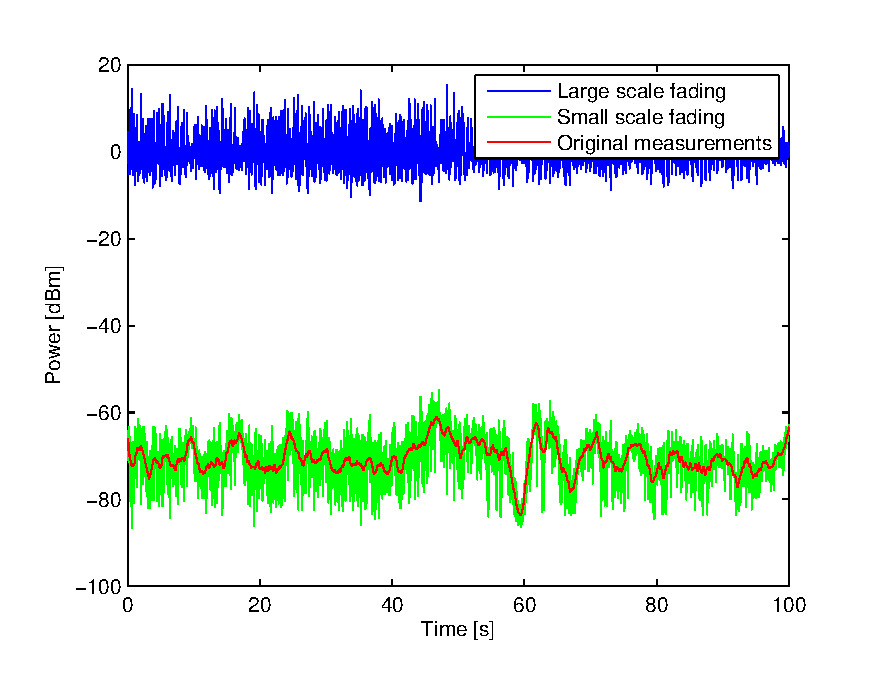
\includegraphics{task1.eps}
%    \caption{Autocorrelation function of Jakes Doppler shift from 3 different realizations.}
%    \label{fig:autocr}
%\end{figure}
As the plow shows, the sum-of-sinusoids are fits the theoretical bessel function better than the internal matlab function based on filters. 


\section{Problem 2}
In this problem we were supposed to simulate a MIMO channel using a Kronecker MIMO channel model, and plot the mean capacity over a SNR range with low, medium and high correlation scenarious. 


%\begin{figure}[h]
%    \centering
%    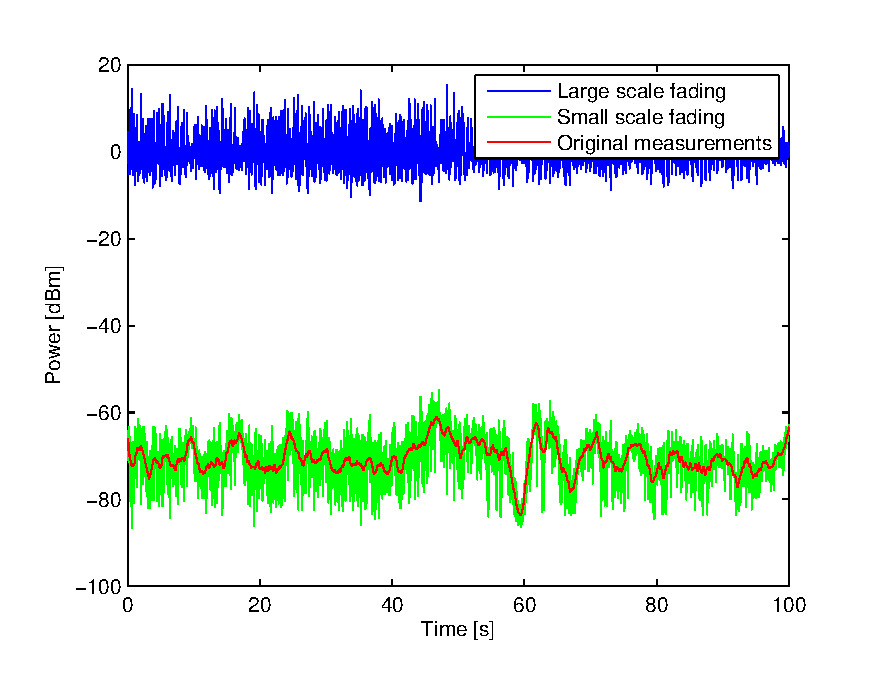
\includegraphics{task1.eps}
%    \caption{Autocorrelation function of Jakes Doppler shift from 3 different realizations.}
%    \label{fig:autocr}
%\end{figure}

\section{Code}

\begin{lstlisting}
close all 
% Lab 3: Radio Engineering
% Eurecom
% Henning Schei

%% Problem 1 


T_S = 1/(7.68e6);
omega_max = 300;
nb_samples = 10e-3 * 7.68e6;


% Generation of narrowband Rayleigh fading Channel
% using internal filter based MATLAB function

rayChanObj = rayleighchan(T_S, omega_max, 0, 0) ;
rayChanObj.StoreHistory = 1;
x = ones(nb_samples,1);
y = filter(rayChanObj,x);
g = rayChanObj.PathGains;

%-------------------------------------------------

% Rayleigh fading channel using Sum of sinusoids method
[acf_sos,lag_sos] = xcorr(sumofsinusoids((1/(7.68e6)), 20, 300,nb_samples));

% Rayleigh fading channel using filter based method
[acf_flt,lag_flt] = xcorr(y);



% Plotting
subplot(1,3,1)
plot(lag_sos,acf_sos/max(acf_sos));
title 'Sum of sinusoids'
subplot(1,3,2)
plot(lag_flt,acf_flt/max(acf_flt));
title 'Filter based method'
chlen = -0.01:T_S:0.01;
subplot(1,3,3)
plot(linspace(-76799,76799,length(besselj(0, 2*pi*300*chlen))),besselj(0, 2*pi*300*chlen));
title 'Theorethical'
figure; 
plot(lag_sos,acf_sos/max(acf_sos), 'r');
hold on
grid on
plot(lag_flt,acf_flt/max(acf_flt),'g');
hold on
plot(linspace(-76799,76799,length(besselj(0, 2*pi*300*chlen))),besselj(0, 2*pi*300*chlen));
title 'Problem one'
legend('Sum-of-Sinusoids', 'Filter based', 'Bessel function'  );
hold off








%% Problem 2

% Generate four independent fading channels 

a = [0 0.3 0.9]; b = [0 0.9 0.9];
G = zeros(2,2,nb_samples);
tmp = sumofsinusoids((1/(7.68e6)), 20, 300,nb_samples);

for k=1:2
    for j=1:2
        for i= 1:length(sumofsinusoids((1/(7.68e6)), 20, 300,nb_samples))
            G(k,j,i) = tmp(i);
        end
        tmp = sumofsinusoids((1/(7.68e6)), 20, 300,nb_samples);
    end
end

Rtx1 = [1 a(1); conj(a(1)) 1] ; Rrx1 = [1 b(1); conj(b(1)) 1];
Rtx2 = [1 a(2); conj(a(2)) 1] ; Rrx2 = [1 b(2); conj(b(2)) 1];
Rtx3 = [1 a(3); conj(a(3)) 1] ; Rrx3 = [1 b(3); conj(b(3)) 1];

H = zeros(2,2,nb_samples);
%H2 = zeros(2,2,nb_samples);
%H3 = zeros(2,2,nb_samples);

% for n =1:length(G)
%     H1(:,:,n) = sqrtm(Rrx1) .* G(:,:,n) .*transpose(sqrtm(Rtx1));
%     H2(:,:,n) = sqrtm(Rrx2) .* G(:,:,n) .*transpose(sqrtm(Rtx2));
%     H3(:,:,n) = sqrtm(Rrx3) .* G(:,:,n) .*transpose(sqrtm(Rtx3));
% end


SNR = power(10,-20/10):10:power(10,30/10);

figure; 
colors = ['b', 'r', 'c'];
tic
for k = 1:3
    R_tx = sqrtm([1 a(k); conj(a(k)) 1]);
    R_rx = sqrtm([1 b(k); conj(b(k)) 1]);
    for m = 1:nb_samples
        H(:,:,m) = R_rx .* G(:,:,m).* transpose(R_tx);
    end
    CAP      = capacity_SU_CL_ML(H,SNR);
    CAP_mean = mean(CAP,2) ;
    plot(SNR, CAP_mean(:), colors(k));
    hold on
end

xlabel('SNR [dB]');
ylabel('Channel Capacity');
title('SNR vs Channel capacity with low, medium, and high correlation');
legend('Low correlation (alpha=0, beta=0)', ...
    'Medium correlation (alpha=0.3, beta=0.9)',...
    'High correlation (alpha=0.9, beta=0.9)');
    
toc










% figure;
% 
% 
% [CAP] = capacity_SU_CL_ML( H1, SNR ,0);
% plot(SNR,CAP);
% 
% figure;
% title 'Capacity of SU MIMO channel for medium correlation case';
% for i=1:10:length(SNR)
%     [CAP] = capacity_SU_CL_ML( H2, SNR(i),0);
%     hold on
%     plot(CAP);
% end
% figure;
% title 'Capacity of SU MIMO channel for high correlation case';
% for i=1:10:length(SNR)
%     [CAP] = capacity_SU_CL_ML( H3, SNR(i),0);
%     hold on
%     plot(CAP);
% end






\end{lstlisting}
 

\end{document}
